\section{Architektura}

Cílem bylo vytvořit aplikaci, která bude mít jako hlavní ovládací prvek mobilní telefon. Kvůli různým typům mobilních telefonů nemůžeme spoléhat na to, že každý telefon dokáže rozpoznávat objekty z vyfocených obrázků, takže bylo nutné přidat i backendový server. Tento server musí být schopný zpracovávat obrázky a rozpoznávat co se na nich nachází. Kvůli tomu, že všechna zařízení se připojují na backend tak je potřeba rozlišovat uživatele. Kvůli tomu zde musí běžet databáze pro ukládání data a pro přidání rychlosti také cache, která zmenší dotazování do hlavní databáze. Pro resetování hesel musí být backend schopný zasílat emaily. \par
Pro snazší zadávání úkolů a zobrazování jak se úkol podařilo splnit bylo potřeba přidat další zařízení které by se o to staralo. Pro toto zobrazování byl vybrán webový prohlížeč, do kterého se hráč přihlásí stejným účtem jako na telefonu a spustí se mu v něm hra, ve které bude zde schopen sledovat zadání svých úkolů.
%//TODO CDN?

\begin{figure}[h]
    \centering
    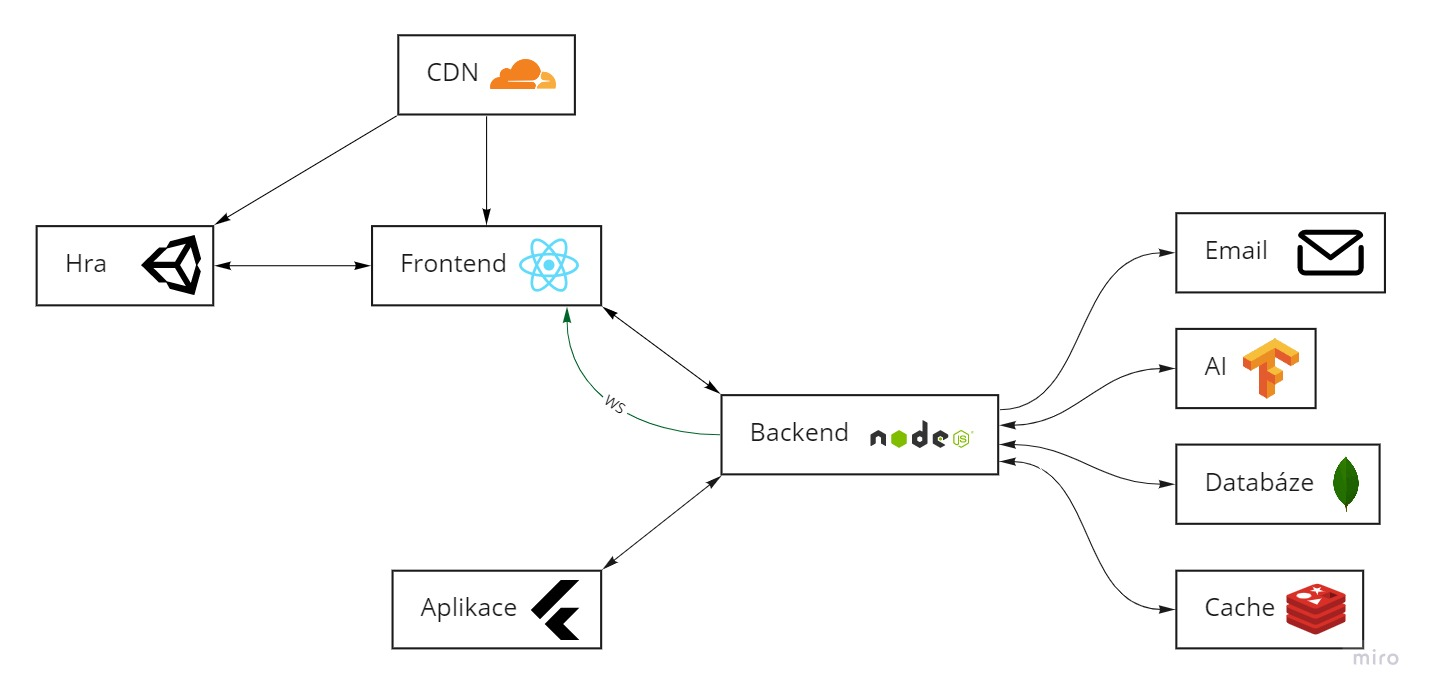
\includegraphics[width=0.6\textwidth]{img/architektura.jpg}
    \caption{Architektura aplikace.}
    \label{fig:architektura}
\end{figure}